\documentclass[a4paper,12pt]{amsart}

\usepackage{pdfpages}
\usepackage{graphicx}
\usepackage{amsmath}
\usepackage{amsfonts}
\usepackage{amssymb}
\usepackage[margin=0.6in]{geometry}
\usepackage[utf8]{inputenc}
\usepackage{multirow}

\begin{document}

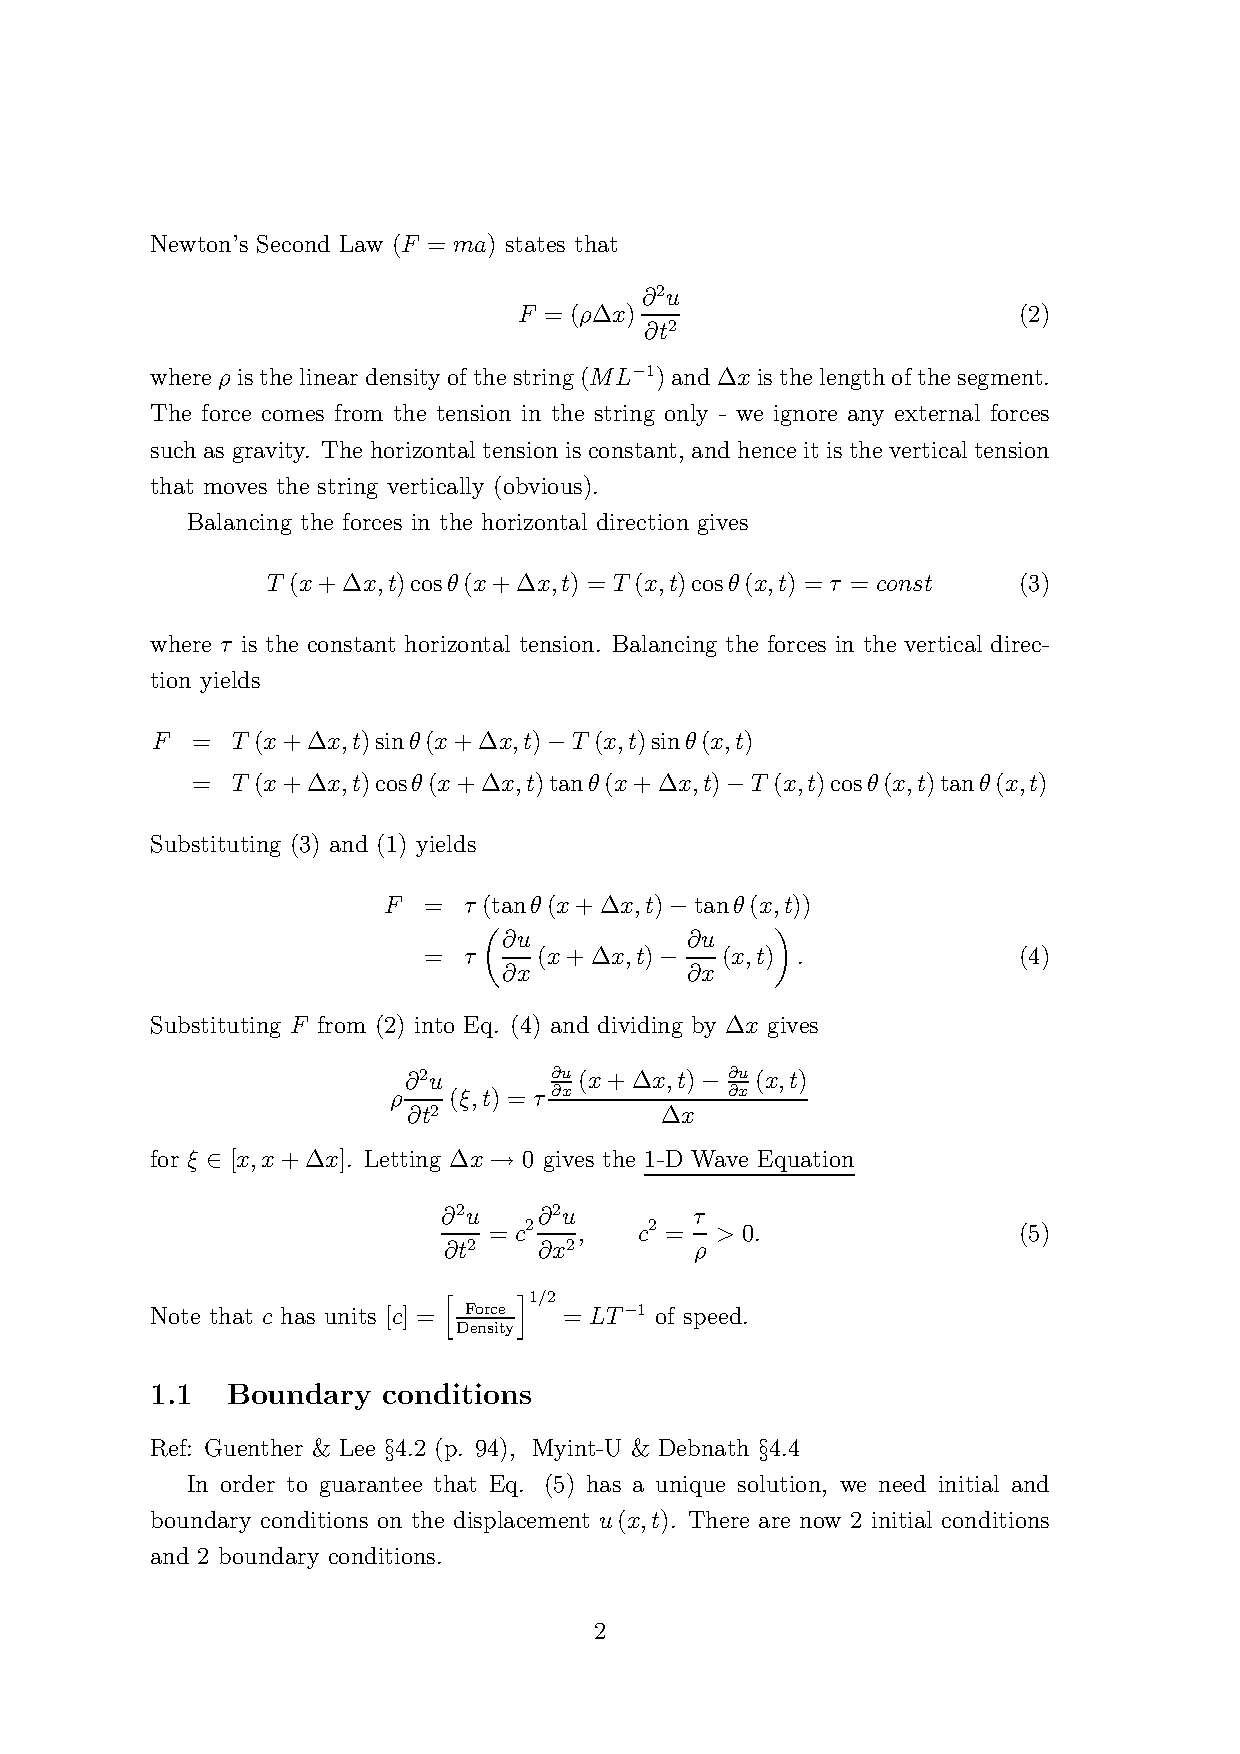
\includepdf[pages=-,pagecommand={},width=\textwidth]{../normal_pdf.pdf}
\newpage

Newton's Second Law $(F=m a)$ states that
$$
F=(\rho \Delta x) \frac{\partial^{2} u}{\partial t^{2}}
$$
where $\rho$ is the linear density of the string $\left(M L^{-1}\right)$ and $\Delta x$ is the length of the segment. The force comes from the tension in the string only - we ignore any external forces such as gravity. The horizontal tension is constant, and hence it is the vertical tension that moves the string vertically (obvious). Balancing the forces in the horizontal direction gives
$$
T(x+\Delta x, t) \cos \theta(x+\Delta x, t)=T(x, t) \cos \theta(x, t)=\tau=\mathrm{const}
$$
where $\tau$ is the constant horizontal tension. Balancing the forces in the vertical direction yields
$F=T(x+\Delta x, t) \sin \theta(x+\Delta x, t)-T(x, t) \sin \theta(x, t)$
$=T(x+\Delta x, t) \cos \theta(x+\Delta x, t) \tan \theta(x+\Delta x, t)-T(x, t) \cos \theta(x, t) \tan \theta(x, t)$
Substituting ( 3) and (1) yields
$$
\begin{aligned}
F &=\tau(\tan \theta(x+\Delta x, t)-\tan \theta(x, t)) \\
&=\tau\left(\frac{\partial u}{\partial x}(x+\Delta x, t)-\frac{\partial u}{\partial x}(x, t)\right)
\end{aligned}
$$
Substituting $F$ from ( 2 ) into Eq. (4) and dividing by $\Delta x$ gives
$$
\rho \frac{\partial^{2} u}{\partial t^{2}}(\xi, t)=\tau \frac{\frac{\partial u}{\partial x}(x+\Delta x, t)-\frac{\partial u}{\partial x}(x, t)}{\Delta x}
$$
for $\xi \in[x, x+\Delta x] .$ Letting $\Delta x \rightarrow 0$ gives the 1 -D Wave Equation
$$
\frac{\partial^{2} u}{\partial t^{2}}=c^{2} \frac{\partial^{2} u}{\partial x^{2}}, \quad c^{2}=\frac{\tau}{\rho}>0
$$
Note that $c$ has units $[c]=\left[\frac{\text { Forree }}{\text { Density }}\right]^{1 / 2}=L T^{-1}$ of speed.
1.1 Boundary conditions
Ref: Guenther \& Lee $\$ 4.2 \text { (p. } 94),$ Myint-U \& Debnath $\$ 4.4$ In order to guarantee that Eq. (5) has a unique solution, we need initial and boundary conditions on the displacement $u(x, t) .$ There are now 2 initial conditions and 2 boundary conditions.

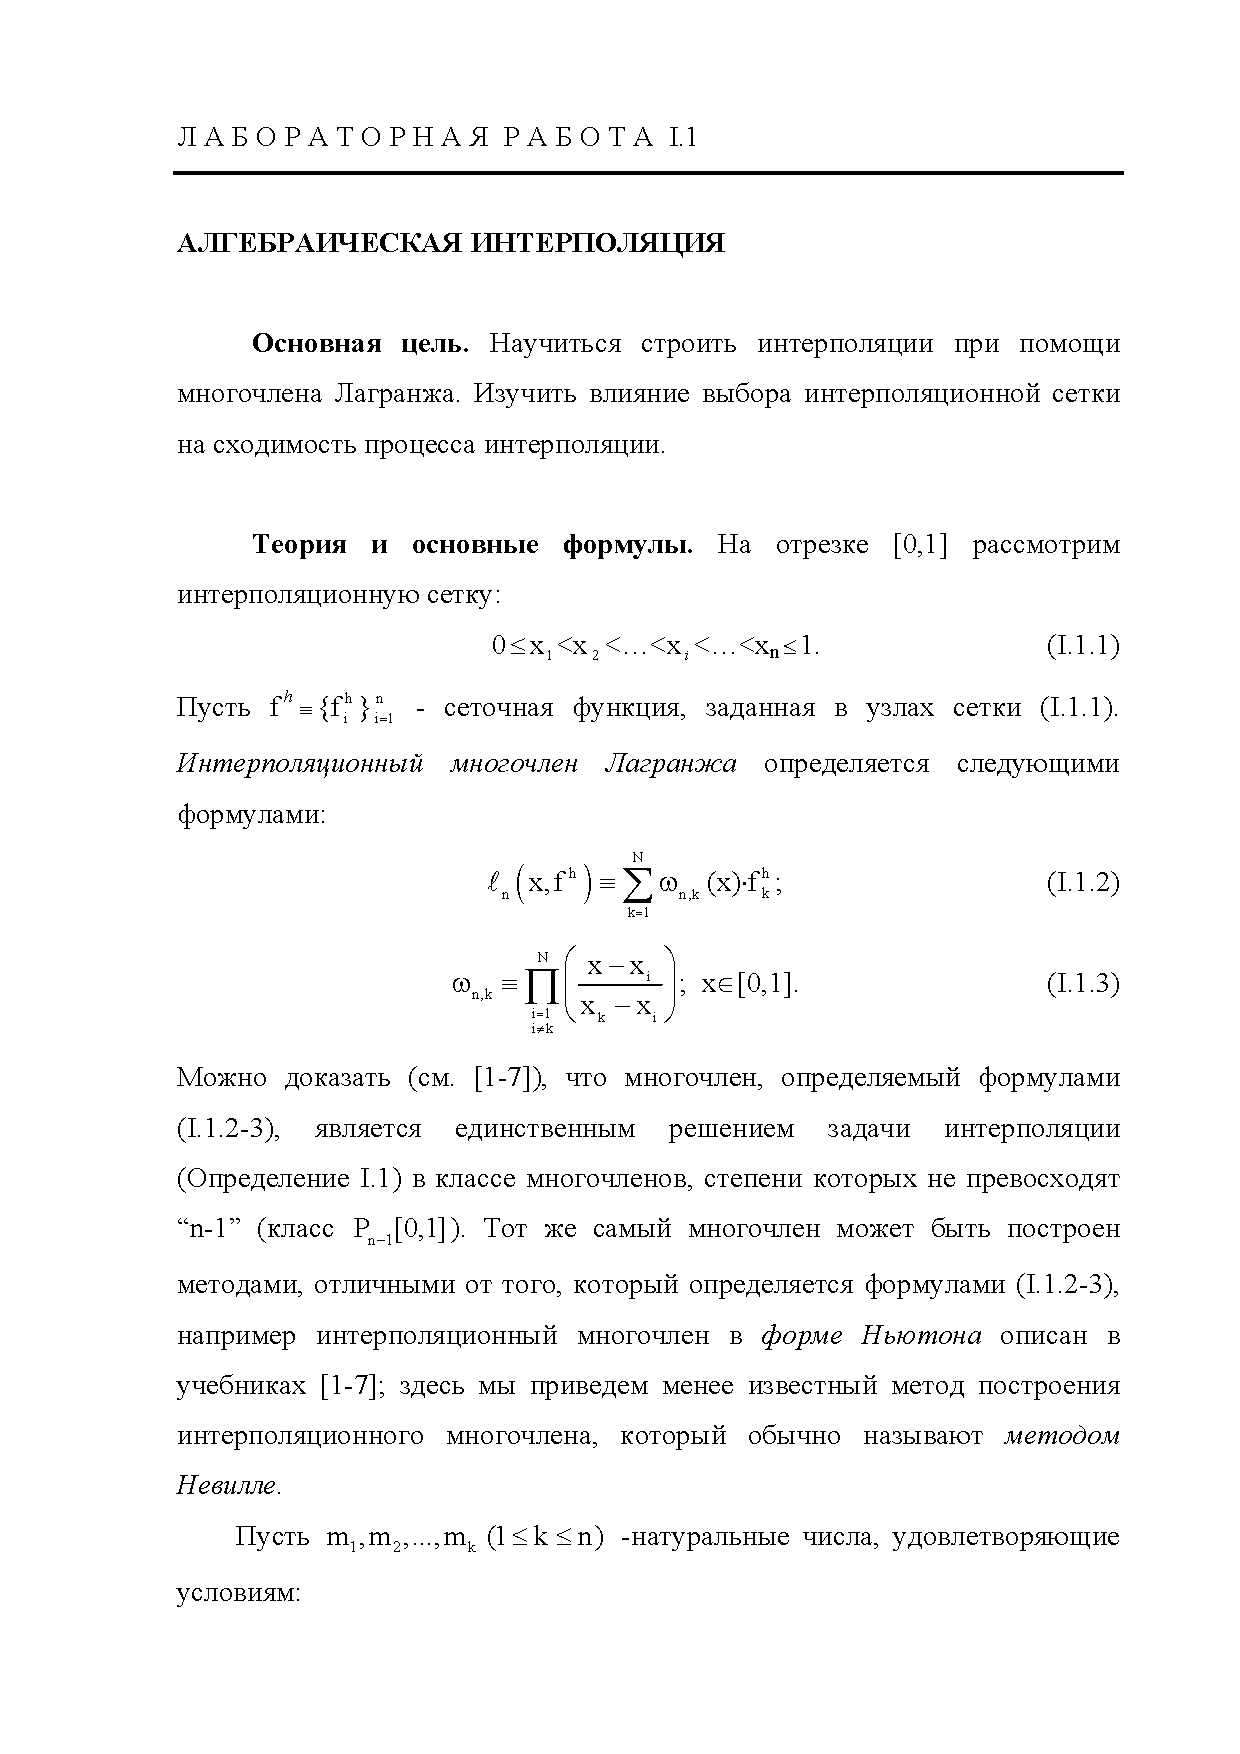
\includepdf[pages=-,pagecommand={},width=\textwidth]{../russian.pdf}
\newpage

IA 5 O PA TOPHA $\$$ PA 5 O TA 1.1
Nricsewurcckus unirepootatuar
Ochoshas ueas. Hayurrbca crpouts untepnotialuhu npu nomoun MHorowneha JarpaHxka. Hayurntb BIHAHHe BLIGopa HHTepnonguhoHHoù ceTKH Ha cxoaumocts npouecca HHTepnonsuuh.
Teopua n ocuosmble phiopuyabl. Ha orpeske [0,1] paccurorphy HHrepnotaluromylo cerry: $$ 0 \leq x_{1}<x_{2}<\ldots<x_{1}<\ldots<x_{n} \leq 1 $$ Hyctb $f^{4}=\left\{f_{1}^{4}\right\}_{4}^{2}$ - cerounar phiynkilus , andawnar $B$ yarax cerxu (I.1.1). Humepnouratuonnbili nuceoutren Jazpanaca onpezeraetes creayiounsm phiopuyaamı:
$$
\begin{array}{l}
\text { anozouten Jazpanoxca onpezeraetes creayiouuntur } \\
\qquad \ell_{n}\left(x, f^{n}\right)=\sum_{k=1}^{n} \omega_{n, x}(x) \cdot f_{k}^{*} \\
\omega_{e x} \equiv \prod_{i=1}^{\infty}\left(\frac{x-x_{i}}{x_{k}-x_{i}}\right) ; x \in[0,1]
\end{array}
$$
Moxko Aoka3arb (cM. [1-7]), "To Mnoroutinen, onpezenzesibuiù phiopuynaun
(1.1.2-3), samates eauncracumbly pemennem 3añaun nurrepnotiauun (OnpeñeneHue
I.1) B KIacce struorotutenos, creneun Kotopblx He npegocxourt "n-1" (kracc
P\_-L[0,1]). Tot we caubsiu $\mathrm{ MAOro*atel } \text { Moxer } 6 \text
{ brib noctpoen }$
Meto\_laMH, OTIM4HLIMH OT TOTO, KOTOPLIÜ onpe,TeTSETCS QopMy. nanpumep merepnotisumounbili menter apwere Hbomona omucan $\mathbf{B}$ yue6Hukax $[1-7] ;$ 37ecb Mbl npusezen MeHee H3BeCTHbIù MeTOA nocrpoeHus
HHTeprotsunohhoro mHorouneua, kotopbili o6blyHo HazbIBaroT Memodom Hesuzze.
IIycts $\mathrm{m}_{1}, \mathrm{m}_{2}, \ldots, \mathrm{m}_{\mathrm{k}}(1 \leq \mathrm{k} \leq \mathrm{n})$ - - HarypaTsHble unc-aa, y Aosiersopaioume
yctoBHSM:

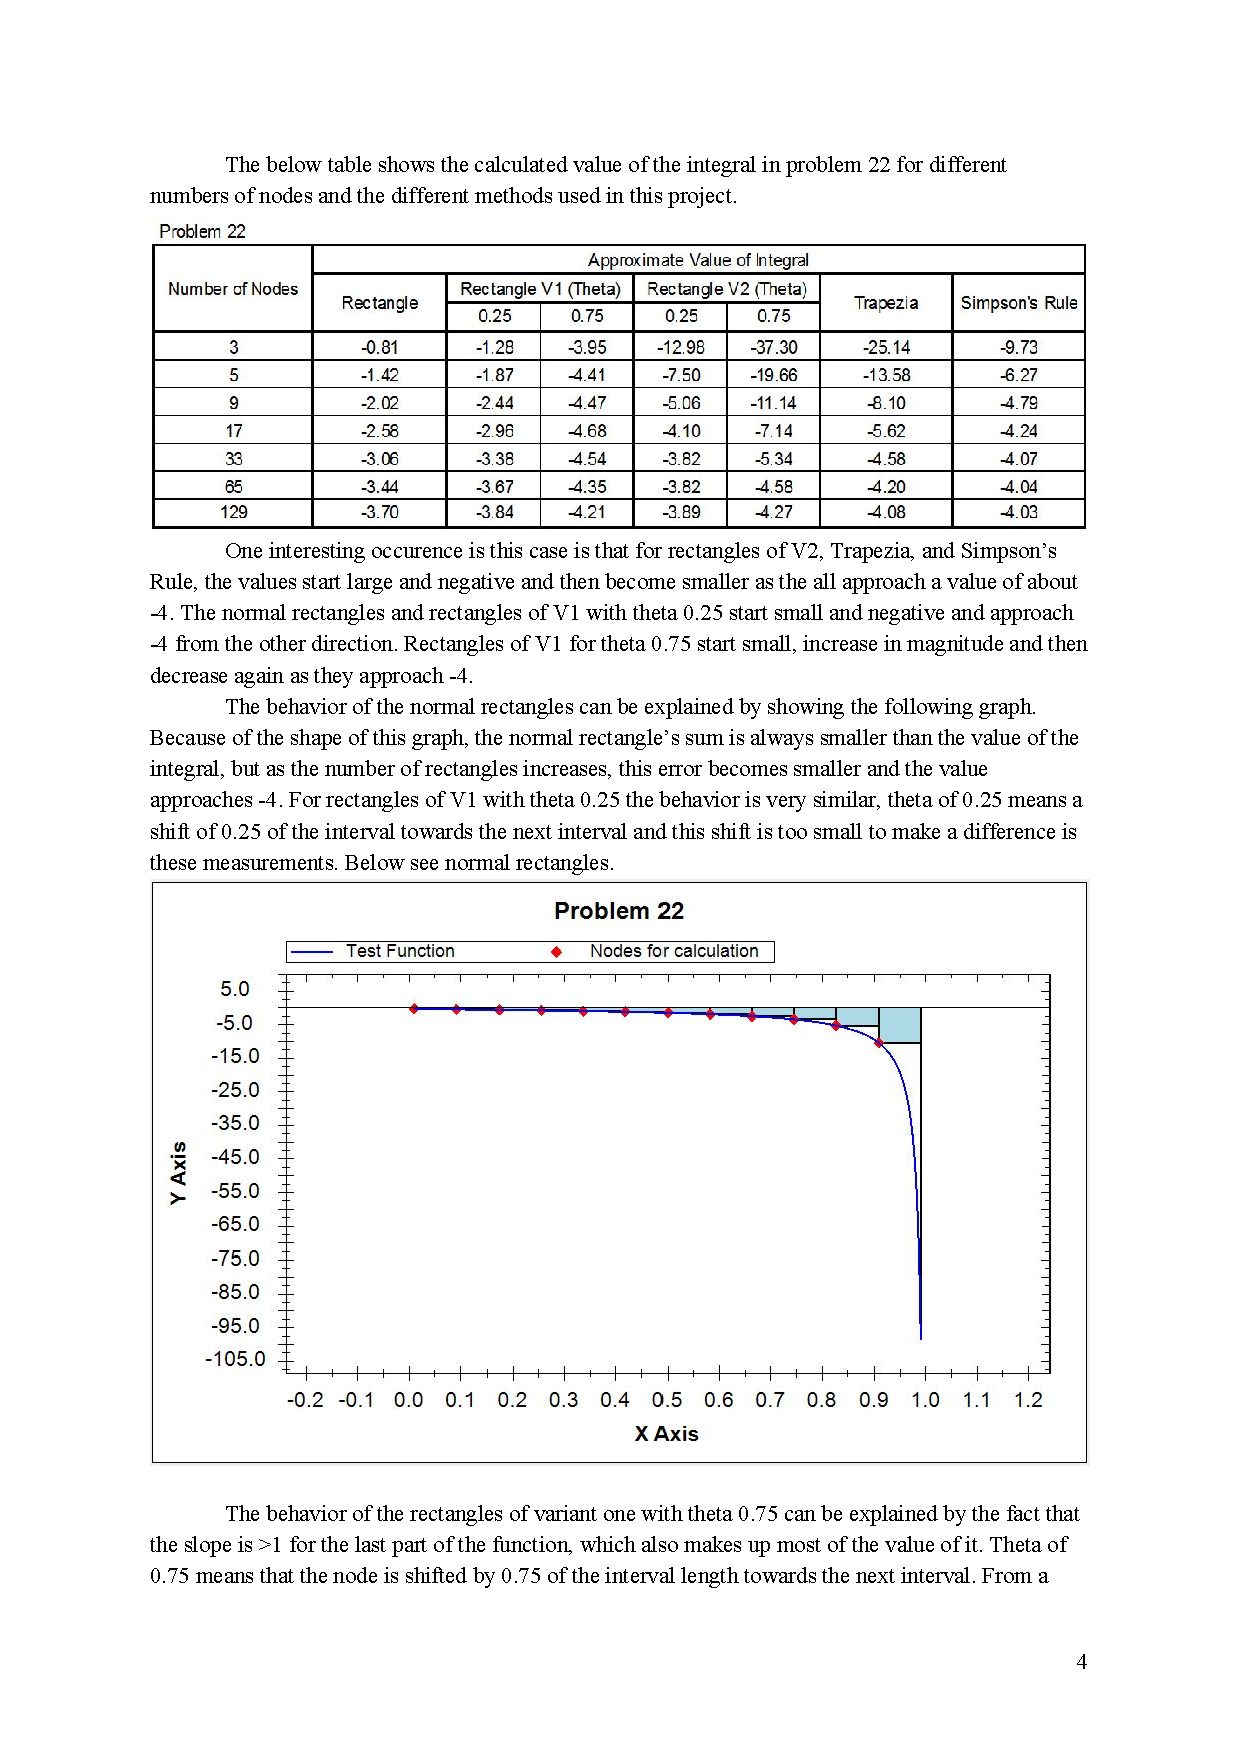
\includepdf[pages=-,pagecommand={},width=\textwidth]{../graph_table.pdf}
\newpage

The below table shows the calculated value of the integral in problem 22 for different numbers of nodes and the different methods used in this project.
\begin{tabular}{|c|c|c|c|c|c|c|c|}
\hline \multirow{2}{*} { Nimber } & \multicolumn{4}{|c|} { Ampoin } \\
\hline & Recinge & \multicolumn{3}{|c|} { Rectange V(MEder) } \\
\hline & Recturde $V_{2}($ mest & & \\
\hline 3 & -0.81 & 0.25 & 0.75 & 0.73 \\
\hline 5 & -142 & -128 & -395 & -1298 & -37.30 & -2514 & -9.73 \\
\hline 9 & 202 & -187 & +41 & -7.50 & -19.68 & -1358 & 627 \\
\hline 17 & 258 & 244 & 447 & -506 & -11.4 & 8.10 & 4.79 \\
\hline 33 & 325 & 296 & 468 & 410 & -14 & 562 & 424 \\
\hline 65 & 344 & 363 & 454 & 382 & 534 & 458 & 407 \\
\hline 128 & 370 & 384 & 435 & 382 & 458 & 420 & 404 \\
\hline
\end{tabular} One interesting occurence is this case is that for rectangles of $\mathrm{V} 2,$ Traperia, and Simpson's Rule, the values start large and negative and then become smaller as the all approach a value of about
- 4. The normal rectangles and rectangles of $V 1$ with theta 0.25 start small and negative and approach
- 4 from the other direction. Rectangles of $\mathrm{V} 1$ for theta 0.75 start small, increase in magnitude and then decrease again as they approach -4 The behavior of the normal rectangles can be explained by showing the following graph. Because of the shape of this graph, the normal rectangle's sum is always smaller than the value of the integral, but as the number of rectangles increases, this error becomes smaller and the value approaches - 4. For rectangles of V1 with theta 0.25 the behavior is very similar, theta of 0.25 means a \begin{tabular}{|c|}
\hline shift of 0.25 of the interval towards the next interral and this shift is too small to make a difference is \\
these measurements. Below sec normal rectangles. \\
\hline Problem 22 \\
5.0 \\
\hline 5.0 \\
-15.0 \\
-25.0 \\
\hline$=$ Tealfunction \\
-35.0 \\
\hline$\frac{-1}{2}=45.0=$ \\
$\geq \frac{1}{5}=$ \\
255.0 \\
-65.0 \\
-75.0 \\
-85.0 \\
-95.0 \\
-105.0 \\
\hline
\end{tabular}
The behavior of the rectangles of variant one with theta 0.75 can be explained by the fact that the slope is $>1$ for the last part of the function, which also makes up most of the value of it. Theta of
0.75 means that the node is shifted by 0.75 of the interval length towards the next interval. From a

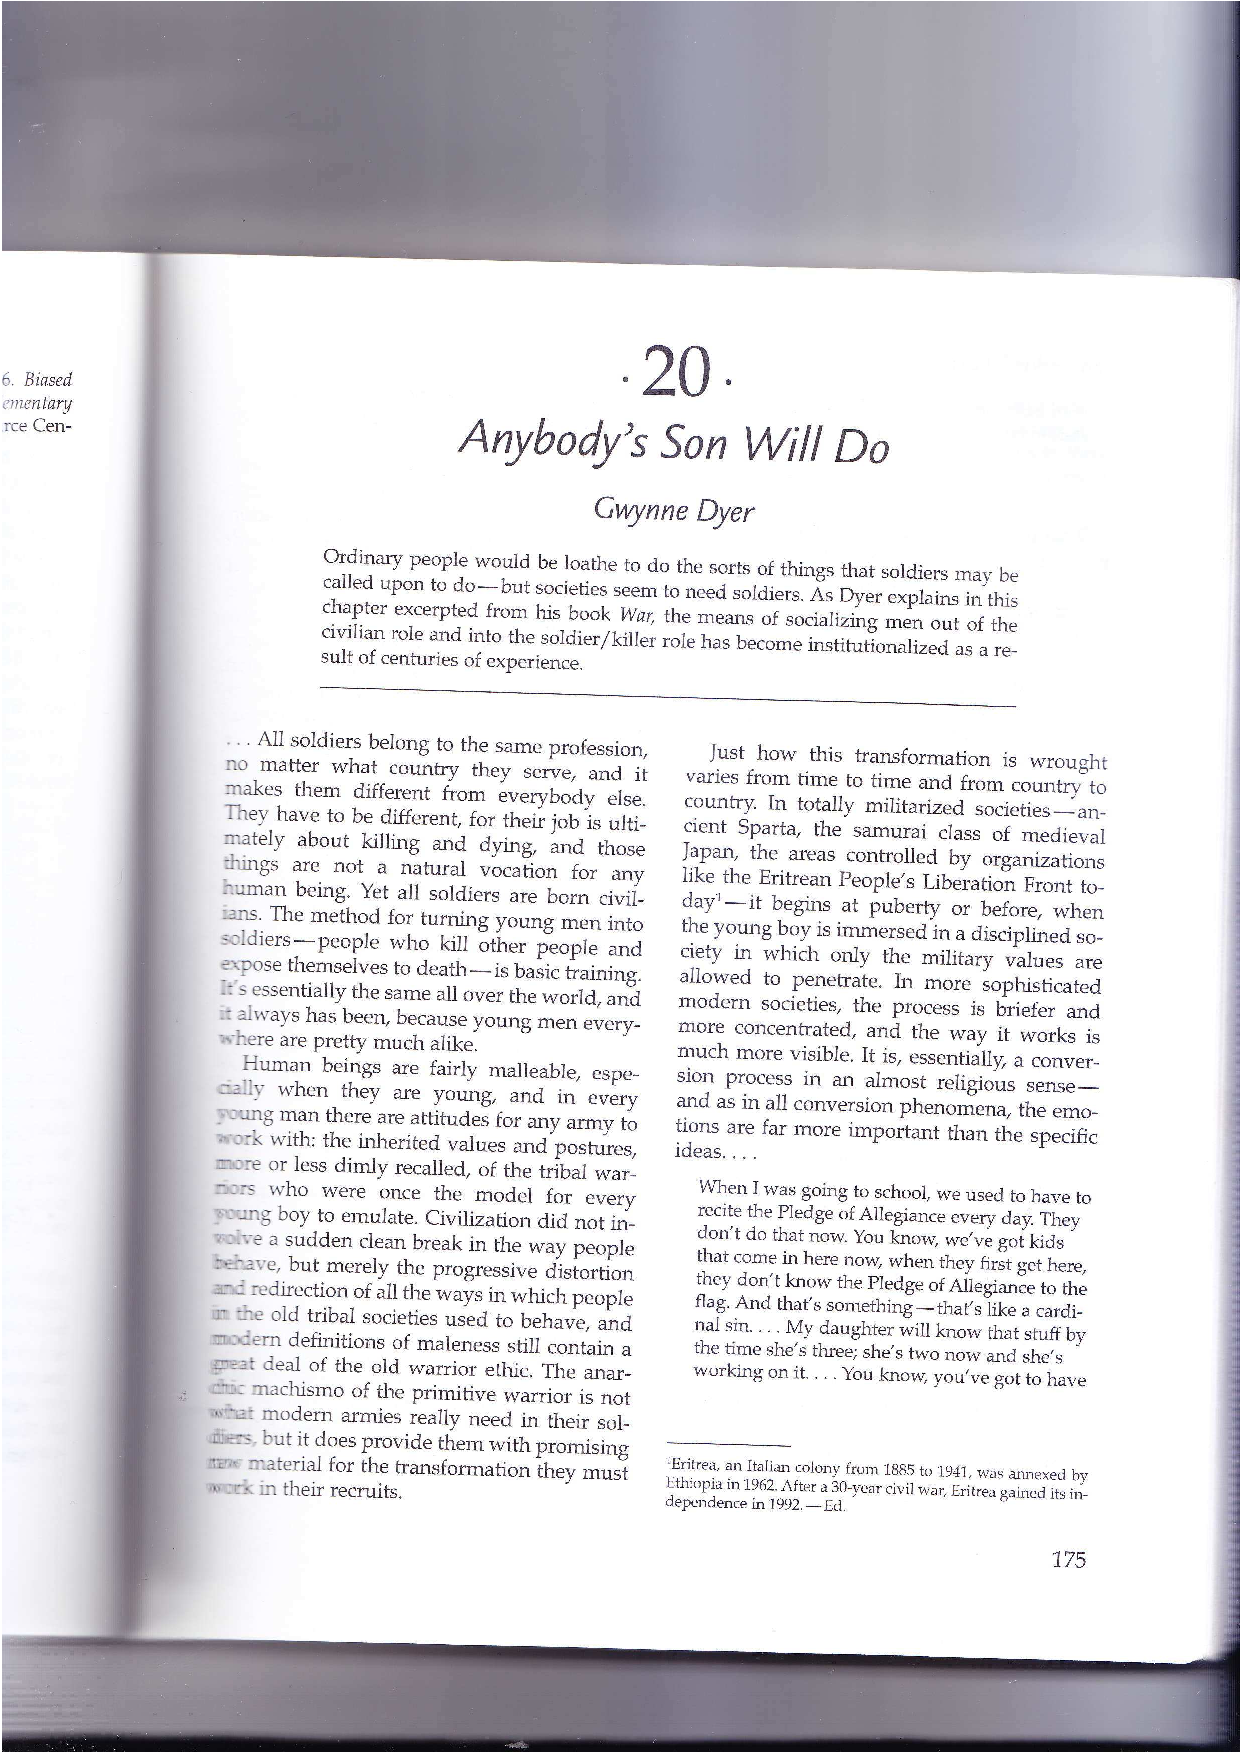
\includepdf[pages=-,pagecommand={},width=\textwidth]{../bad_scan.pdf}
\newpage

.20
Anybody's Son Will Do
cimmenyererer
Ordinary people would be loathe to do the sorts of things that soldiers may be called upon to do - but societies seem to need soldiers. As Dyer explains in this chapter excerpted from his book War, the means of socializing men out of the civilian role and into the soldier/killer role has become institutionalized as a result of centuries of experience.
All soldiers belong to the same profession, $\quad$ Just how this transformation is wrought no matter what country they serve, and it varies from time to time and from country to makes them different from everybody else. country. In totally militarized societies - anThey have to be different, for their job is ulti- - cient Sparta, the samurai class of medieval mately about killing and dying, and those Japan, the areas controlled by organizations things are not a natural vocation for any like the Eritrean People's Liberation Front to:
human being. Yet all soldiers are born civil- day'- it begins at puberty or before, when ians. The method for turning young men into the young boy is immersed in a disciplined sosoldiers- people who kill other people and ciety in which only the military values are expose themselves to death - is basic training. allowed to penetrate. In more sophisticated Ifsessentially the same all over the world, and $\quad$ modern societies, the process is briefer and
italways has been, because young men every- - more concentrated, and the way it works is where are pretty much alike. $\quad$ much more visible. It is, essentially, a converHuman beings are fairly malleable, espe- - sion process in an almost religious sense-
cally when they are young, and in every and as in all conversion phenomena, the emoyoung man there are attitudes for any army to tions are far more important than the specific work with: the inherited values and postures, ideas. more or less dimly recalled, of the tribal war- $\quad$ When I was going to school, we used to have to
nors who were once the model for every $\quad$ recite the Pledge of Allegiance every day. They zoung boy to emulate. Civilization did not in- $\quad$ don't do that now. You know, we've got kids "solve a sudden clean break in the way people $\quad$ that come in here now, when they first get here, behave, but merely the progressive distortion
they don't know the Pledge of Allegiance to the
and redirection of all the ways in which people $\quad$ flag. And that's something - that's like a cardiin the old tribal societies used to behave, and nal sin..... My daughter will know that stuff by modern definitions of maleness still contain a $\quad$ the time she's three; she's two now and she's
Feat deal of the old warrior ethic. The anar- working on it.... You know, you've got to have
tic machismo of the primitive warrior is not
what modern armies really need in their sol-
Giers, but it does provide them with promising
There material for the transformation they must work in their recruits.

\newpage

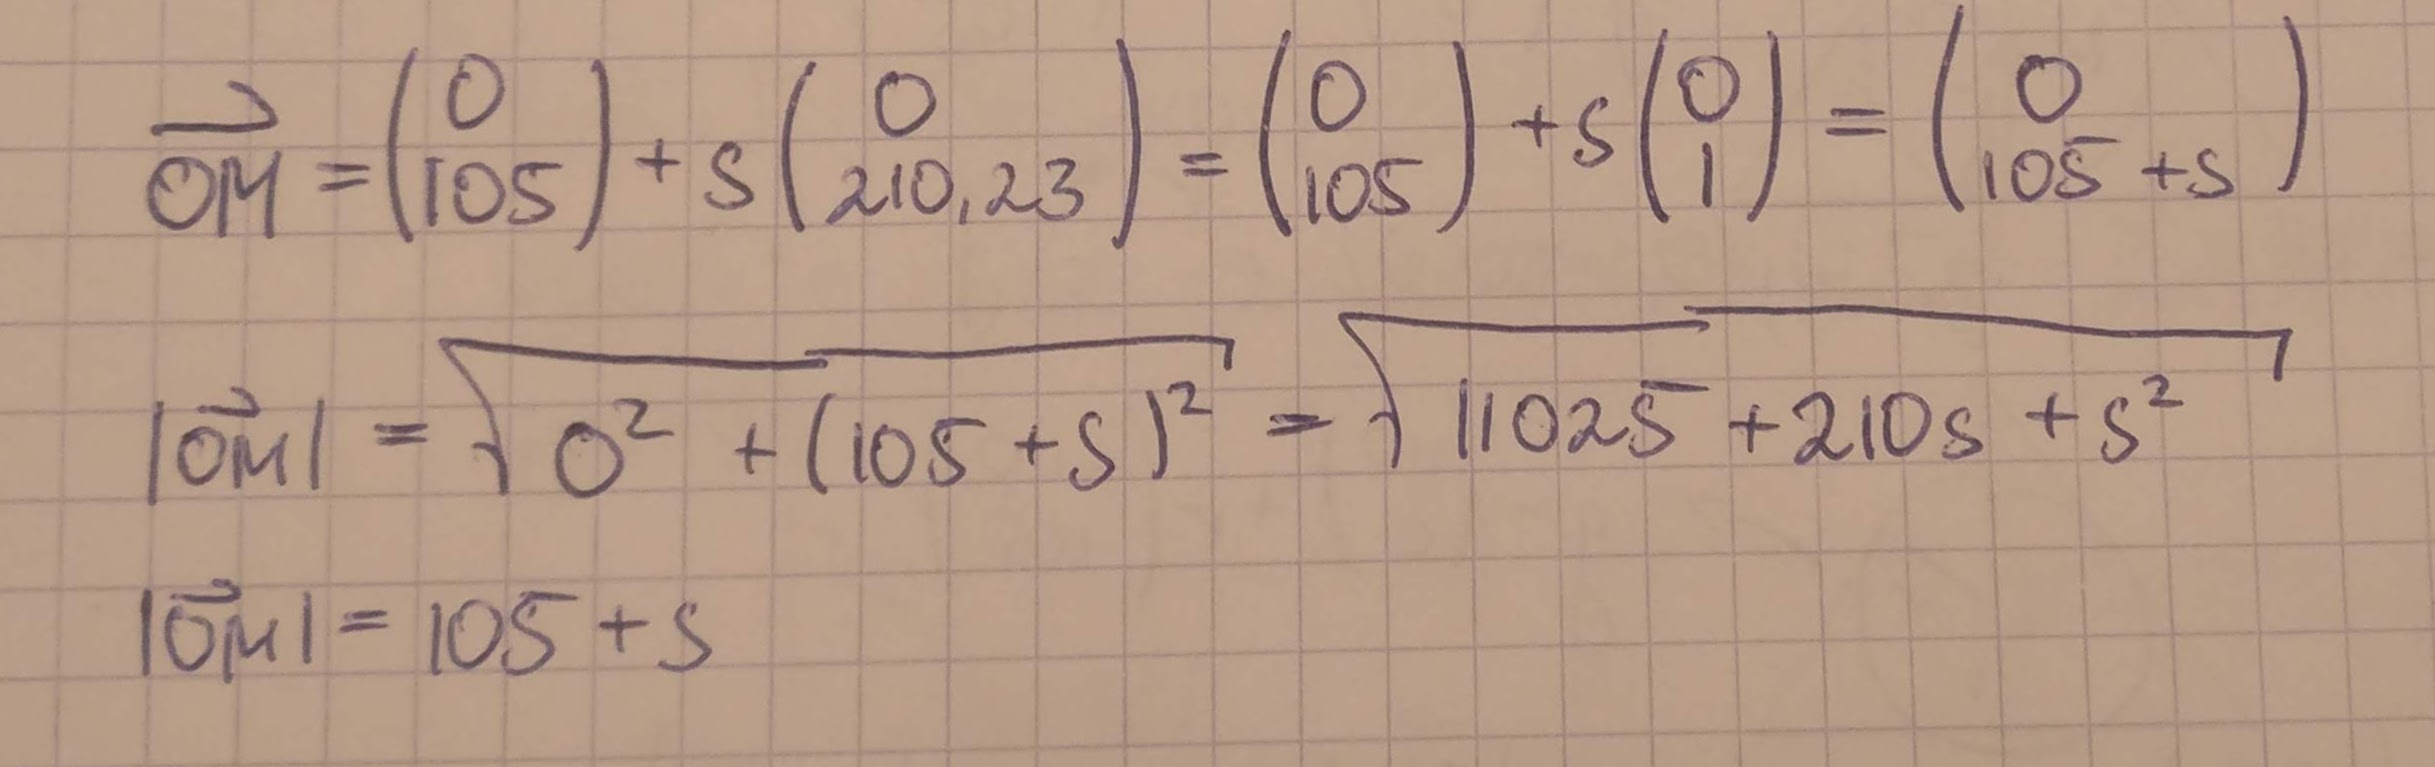
\includegraphics[width=\textwidth]{../handwriting}

\begin{equation}\nonumber
\begin{aligned}
&\overrightarrow{OM}=\left(\begin{array}{l}
0 \\
105
\end{array}\right)+s\left(\begin{array}{c}
0 \\
210,23
\end{array}\right)=\left(\begin{array}{l}
0 \\
105
\end{array}\right)+s\left(\begin{array}{l}
0 \\
1
\end{array}\right)=\left(\begin{array}{l}
0 \\
105+s
\end{array}\right)\\
&|\overrightarrow{OM}|=\sqrt{0^{2}+(105+5)^{2}}=\sqrt{11025}+210 s+s^{2}\\
&|\overrightarrow{OM}|=105
\end{aligned}
\end{equation}

\end{document}
